\cleartooddpage[\thispagestyle{empty}]
\chapter{Gamma Rays and Dark Matter}

As this analysis searches for dark matter from the presence of gamma rays, a discussion on gamma rays and their properties is necessary.
This discussion revolves around three main topics: astrophysical mechanisms for creating gamma rays, the production of gamma rays from the dark matter halo around the Galactic Center, and gamma-ray-induced air showers in the Earth's atmosphere.

\section{Methods of Creation}

  There are three astrophysical mechanisms for gamma ray production at TeV energies.
  The leptonic mechanism is when gamma rays' last energetic interaction is with electrons, while the hadronic mechanism is when gamma rays are created via proton interactions.
  The third mechanism, searched for in this analysis, is when two WIMP dark matter particles annihilate either directly or indirectly into gamma rays.

  In leptonic production, stars and galaxies have their own magnetic fields, and also emit electrons.
  Inverse compton (\cite{compton_effect}) scattering can occur, where electrons and ambient photons collide, transferring energy to the photon.
  After multiple repetitions of this, a small fraction of the original photon population can achieve TeV-scale energies.
  Additionally, electrons spiralling through magnetic fields can produce synchrotron photons with X-Ray energies, meaning fewer inverse compton scatterings are needed to reach TeV energies \cite{self_compton}.

  In hadronic processes, protons are first accelerated by fermi acceleraton, emitted as part of a jet~\cite{hadronic1,hadronic2}, or other mechanisms.
  Then, upon striking an ambient atom, the proton will decay into $\pi^{+}$, $\pi^{-}$, and $\pi^{0}$.
  The $\pi^{0}$ then quickly (<\SI{1}{s}) decays into a $\gamma\gamma$ pair, with \nicetilde $\frac{1}{10}^{\text{th}}$ the original proton's energy.
  Much of the diffuse gamma ray component of the galactic disk is due to extra-galactic high-energy protons colliding with the atoms of the dusty galactic plane \cite{GalacticDiffuseGammaRays}.

  \subsection{Dark Matter Interactions}
    As discussed in various extensions of SUSY, dark matter may be detectable by three general detection schemes, illustrated in Figure \ref{fig:3_searches}.

    % add popular figure for the three detection type
    \begin{figure}[ht]
      \centering
      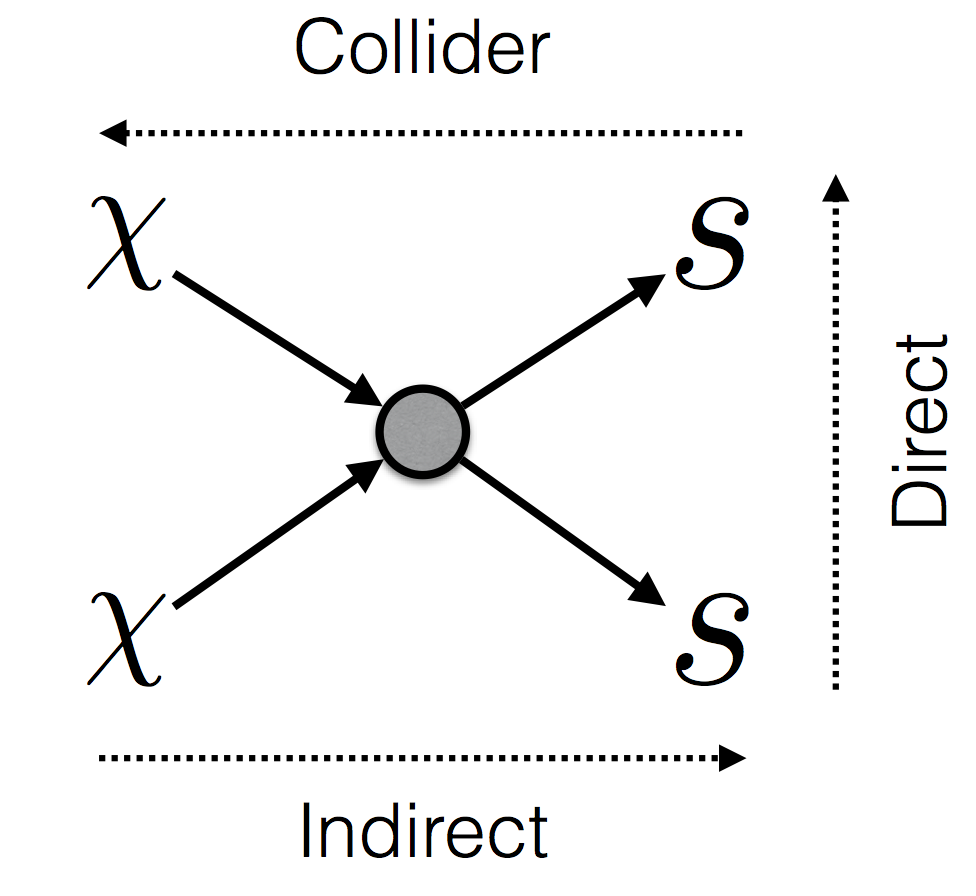
\includegraphics[width=0.45\textwidth]{images/3waystodetect.eps}
      \caption[3 Search Techniques]{
        The three general search techniques for dark matter.}
      \label{fig:3_searches}
    \end{figure}

    In Collider detection, $ss \rightarrow \chi\chi$, standard model particles ($ss$) are accelerated and collide in a detector, and the resulting particle fragments are measured by a slew of measuring equipment.
    A significant milestone was achieved when this technique was used to detect the Higgs boson~\cite{Higgs_ATLAS,Higgs_CMS}.
    Since the properties of the input particles are well-known, and output particles are well measured, the missing remainder may potentially be a dark matter particle.

    With Direct detection, $\chi s \rightarrow \chi s$, sensitive particle detectors are built deep underground, where a dark matter particle impacting against an electron or nuclei creates a detectable recoil.
    Depending on the detector, this recoil can cause a detectable charge, a heat spike, an acoustic vibration, or a visual reaction.
    Often experiments make use of several of these signals, as well as the time difference between each of observable.
    Though to date, no substantial dark matter signal has been detected with these methods~\cite{direct_dm_detection}.

    With Indirect detection, $\chi\chi \rightarrow ss$, astrophysical observations are analyzed for excess standard model particles, unexplained by other astrophysics.
    In this analysis an excess of gamma rays is sought, as the center of our galaxy is believed to host a dark matter halo.
    This spherical halo would allow for many $\chi\chi$ annihilations, producing gamma rays via: 

    $$\chi\bar{\chi} \rightarrow s\bar{s} \rightarrow \gamma\gamma$$

    where $s\bar{s}$ can be any quark or lepton particle-antiparticle pair ($t\bar{t}$, $s\bar{s}$, $e^{-}e^{+}$, etc).
    These different annhilation channels can produce different spectra of gamma rays, which will also vary based on the WIMP mass and cross-section chosen.
    This is described further in Section \ref{dm_spectral}.


\section{Galactic Center}

  The galactic center is a complex region of space, with many astrophysical sources of gamma rays.
  A disk of dust lies along the galactic plane, acting as an interaction medium for diffuse proton cosmic rays.
  Nearby supernova remnants also produce gamma-rays as their expanding shell interacts with ambient dust.
  The immediate area surrounding the galactic center a point-source emitter of gamma rays, though this mechanism is uncertain.

  % black hole
  Through kinematic observations of nearby stars, the galactic center has a supermassive black hole, with a mass of \SI{4e6}{\Msol}~\cite{sgra_massdist}.
  The Galactic Center also is a source of \TeV{} gamma rays, though the mechanism that produces them is still under debate.
  One possibility is that the supermassive black hole accelerates protons to PeV energies, which convert into TeV gamma rays~\cite{gc_pevatron}.
  The second possibility suggests a nearby Pulsar Wind Nebula may be providing the gamma-ray-parent particles~\cite{gc_pulsars}.
  While the Galactic Center emits gamma rays, this emission is point-like to ground-based gamma ray telescopes. {\color{red}(rewrite this!?? citation??)}
  This analysis instead focuses on the gamma ray flux outside this point-like inner angular region.

  The disk of gas present in the galactic plane acts as an interaction medium for passing cosmic rays, both from nearby galactic accelerators and from extragalactic sources.
  {\color{red}(discuss diffuse emission??)}

  {\color{red}(somewhere in thesis cite something from each defense committee member!)}

\section{Indirect Dark Matter Detection}
  For this analysis, it is important to understand how a terrestrial telescope like VERITAS can detect the presence of dark matter.
  This is done through indirect detection: observation of the gamma-rays that are emitted when two dark matter particles annihilate.
  As the rate of annihilation depends on the local dark matter number/volume density, the radially-changing structure of dark matter halos also affects the analysis.

  \subsection{Dark Matter and Gamma Rays}
    WIMPs are predicted to decay and self-annihilate into standard model particles.
    Primarily, indirect searches focus on annihilating WIMPs, as the predicted WIMP decay lifetime produces a lower flux of standard model particles than annihilation.
    WIMPs may annihilate into any standard model particle, but most studies examine a WIMP annihilating into a quark-antiquark pair, or a pair of gamma-ray photons.

    For example, two annihilating WIMPs may produce a $t\bar{t}$ pair, which then decays into... {\color{red}??}.
    Or, they may produce $b\bar{b}$, or $\gamma\gamma$.

    These different annihilations will produce different spectra of final gamma rays.
  
  \subsection{Dark Matter Halo Structure}\label{dm_spatial}
    From observations, most galactic dark matter halos can be modeled by several similar density profiles {\color{red}(explain??)}.
    A currently favored profile is the Einasto profile~\cite{einastoprofile1,einastoprofile2}.
    This profile describes the mass/volume density of dark matter at a distance r from the halo center, $\rho(r)$.
    The Einasto profile has the form

    \begin{equation} \label{eqn:einasto}
      \rho_{DM} \left( r \right) = \rho_{s} Exp \left( - \frac{2}{\alpha} \left( {\left( \frac{r}{r_s} \right)}^{\alpha} - 1 \right) \right)
    \end{equation}
    
    where $\alpha$ is taken to be 0.17, from~\cite{PieriGalaxySims}.

    Other profiles exist, but for this analysis only the Einasto profile is used.
    Most simulations show that density profiles should terminate in a sharp peak at $r=0$, but observations of dwarf galaxies instead favor a flat core within a given radius~\cite{CoreVsCusp}.
    For simplicity in this initial analysis, no core radius is applied.
    
    The distance to the galactic center is fixed at \SI{8}{kpc}~\cite{gc_distance_1,gc_distance_2,gc_distance_3}, and the local estimated dark matter mass density is fixed at \SI{0.4}{\GeV\per\cm^3}~\cite{local_dm_density}, though this varies depending on the assumed Milky Way mass profile~\cite{direct_dm_astrophysical_uncertainties}.
    A scale radius $r_s$ of \SI{15.4}{kpc} {\color{red}(cite??)} is also used, and the Einasto profile for the the galactic center halo is shown in Figure \ref{fig:gchalo_density}.
  
    \begin{figure}[ht]
      \centering
      \includegraphics[width=0.95\textwidth]{images/halo/gc_einasto_profile.eps}
      \caption[Galactic Center Einasto Halo Density]{
        Mass density of the dark matter halo used in this analysis.}
      \label{fig:gchalo_density}
    \end{figure}
    
    These profiles can then be used to calculate the spatial distribution of gamma-rays.
    For annihilating dark matter, $\rho\left(r\right)^2$ must be integrated along the line of sight.
    To calculate the amount of gamma rays produced by these annihilations, Equation \ref{eqn:dmflux} can be used.
    
    \begin{equation}\label{eqn:dmflux}
      \frac{ d\Phi }{ dE d \Omega } = \frac{ \left \langle \sigma v \right \rangle }{8 \pi m_\chi^2} \frac{dN_{\gamma}}{dE} \int \rho^2 dl
    \end{equation}
    
    In this, the photon flux $\Phi$ is the number of gamma-ray photons detected per area and per time.
    $\left \langle \sigma v \right \rangle$ is the velocity-averaged cross-section of the dark matter candidate.
    The velocity-averaging is used because the cross-section may be velocity dependent, and the WIMP particles within the halo probably posesses a distribution of velocities.
    The $\frac{dN_{\gamma}}{dE}$ is the spectrum of photons produced by a single $\chi\chi$ annihilation.
    
    \begin{figure}[ht]
    \centering
      \includegraphics[width=0.95\textwidth]{images/halo/gc_einasto_jfactor.eps}
      \caption[Galactic Center Einasto Halo Jfactor]{
        J-factor profile as a function of angle from the galactic center.
        J-factor values are calculated with an integration angle of ${0.01}^{\circ}$.
        {\color{red}Y axis label??}
      }
      \label{fig:gchalo_jfactor}
    \end{figure}
    
    Additionally, simulations of galaxy formation indicate that the presence of baryons diffuses {\color{red}(??)} the central cusp of particles in a potential well {\color{red}(cite??)}.
    This create a central area of constant density in the profile called a core.
    However, due to the low amount of mass contained in dark matter in this core region, celestial bodies near galactic center only have their orbital velocity altered a miniscule amount, making it difficult to measure the inner DM core behavior.

    {\color{red}Sommerfield enhancement (??)}

    % from http://www.pnas.org/content/112/40/12264.full.pdf
    
    {\color{red}DM Flux skymap??}
    
  \subsection{Spectrum of Gamma Rays from Dark Matter}\label{dm_spectral}
    In order to calculate the brightness of the dark matter halo in gamma rays, the produced spectrum from each WIMP annihilation must be known.
    Each WIMP annihilation may directly produce two gamma rays, or may instead produce a $b\bar{b}$  or $t\bar{t}$ pair, which then decays into gamma rays {\color{red}(and other possible decay channels?? leptons??)}, called annihilation channels.
    In order to calculate the different produced gamma-ray spectra for each annihilation channel, the software package CLUMPY \cite{CLUMPYcode} is used.
    The spectral models that CLUMPY uses are based on the tables in PPPC 4~\cite{pppc4_dm_spectra}.

    For this analysis, only the simplest annihilation channels are considered, where WIMP annihilations only use one channel, instead of percent mixes of multiple channels.

    \begin{figure}[ht]
      \centering
      \includegraphics[width=0.95\textwidth]{images/spectra/chichi_spectrum.eps}
      \caption[Single Annihilation Spectra]{
        Resultant photon spectra from a single annihilation of WIMP particles at various WIMP masses.}
      \label{fig:chichi_spectrum}
    \end{figure}

    These spectra, then can be combined with the J-factor equation to calculate how many gamma rays are produced by the halo.

    \FloatBarrier
    
    
\section{Atmospheric Showers}

  When a particle strikes an atom of Earth's atmosphere at relativistic velocities, it can set off a cascade of energetic particles called an air shower~\cite{Bethe1934,Klein1999}.
  When the primary particle is a gamma ray, an electron, or a positron, it creates an electromagnetic shower.
  When the primary is a proton or other baryon, it creates a hadronic shower.
  Electromagnetic air showers are started by a high energy (\nicetilde TeV) electron or gamma-ray, and produce a cascade of electrons, positrons, and photons, where initially each successive generation of particles tends to have more particles but less energy per particle than the last.
  The primary gamma ray will interact with an atmospheric atom, producing a $e^{-}e^{+}$ pair, each with roughly half the primary gamma ray's energy.
  The $e^{-}$ and $e^{+}$ will emit some photons through bremstrahlung radiation, until they have \nicetilde \SI{80}{MeV} of kinetic energy, after which energy losses due to ionization dominate, preventing new shower particles from being created \cite{pdg_2014}.
  The photons created during the shower go on to produce more $e^{-}e^{+}$ pairs, though as each newly created particle has less energy than its parent particle, eventually the photons in the shower don't have enough energy to produce additional $e^{-}e^{+}$ pairs.

  As most (\nicetilde 99\%) of detected air showers are due to protons and not gamma rays, understanding the differences between hadronic showers and electromagnetic showers becomes useful in removing unwanted proton air showers and preserving gamma-ray air showers within the reconstruction software, sometimes referred to as gamma-hadron separation.
  Hadronic showers start with a primary \nicetilde TeV proton that interacts with an atmospheric atom.
  This proton then converts into $\pi^{+}$, $\pi^{-}$, and $\pi^{0}$, each with roughly \nicetilde $\frac{1}{3}$ of the initial proton's energy.
  The $\pi^{+}$ and $\pi^{-}$ can travel far from the main axis of the primary particle, then produce $\mu^{+}\nu_{\mu}$ and $\mu^{-}\bar{\nu}_{\mu}$ pairs, respectivly.
  The $\pi^{0}$ quickly decays into $\gamma\gamma$, which then each start their own electromagnetic shower.
  The $\pi^{+}$ and $\pi^{-}$ can have a large transverse momentum (relative to the primary shower axis), and also have longer decay time ($\pi^{\pm}=\;$\SI{3e-8}{s} vs $\pi^{0}=\;$\SI{9e-17}{s} \cite{pdg_2014} ).
  Both of these effects contribute to sub-showers being created further away from the primary particle axis, which tends to cause hadronic showers (and their resulting Cherenkov images) to be wider than a purely electromagnetic shower of the same length. 

  \begin{figure}[ht]
    \centering
    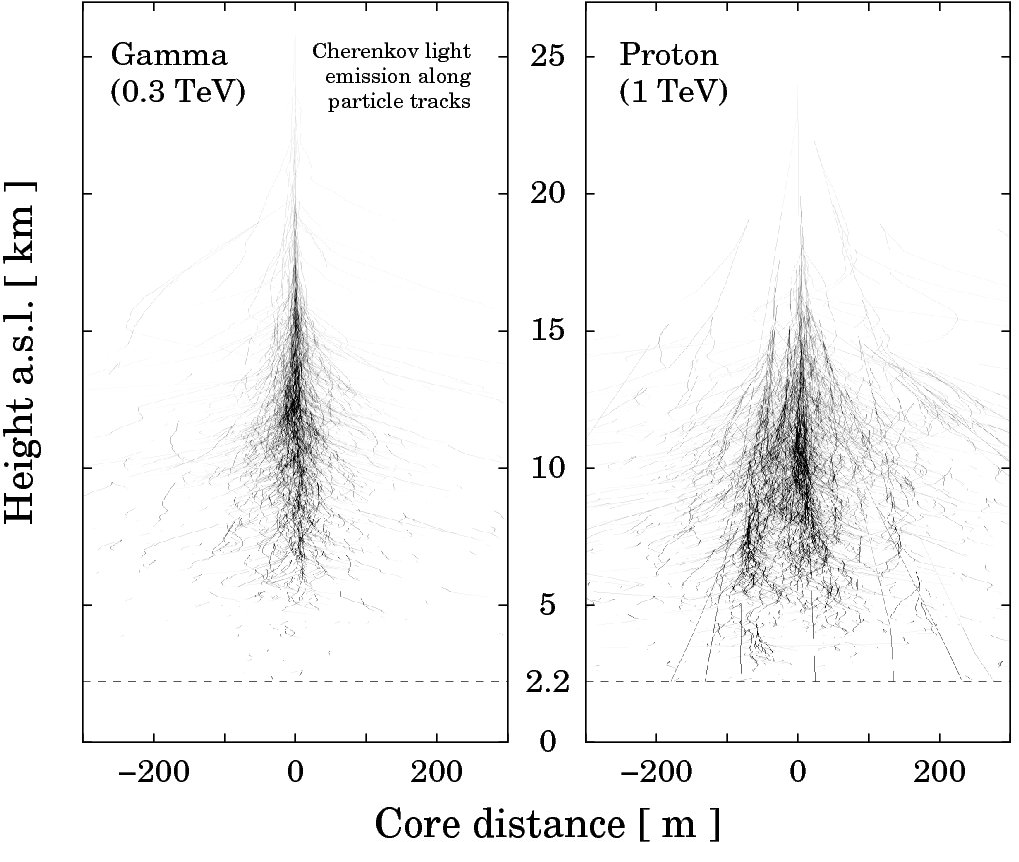
\includegraphics[width=0.95\textwidth]{images/showers_gamma_proton}
    \caption[Gamma Ray and Proton Showers]{
      A gamma ray shower alongside a proton shower~\cite{Bernlohr2008149}.
    }
    \label{fig:gamma_vs_proton_airshower}
  \end{figure}

  \begin{figure}[ht]
    \centering
    \includegraphics[width=0.85\textwidth]{images/cascade_diagram/emcascade.eps}
    \caption[Electromagnetic Cascade]{
      Diagram of an electromagnetic cascade as it decends downwards through the atmosphere, layered by interaction generation.
    }
    \label{fig:emcascade}
  \end{figure}

  \FloatBarrier

  \subsection{Cherenkov Photons}

  Within atmospheric showers, any charged particles travelling at velocity $v > c$ will create Cherenkov photons~\cite{cherenkov}, where $c$ is the speed of light in the atmosphere.
  From a single charged particle of constant velocity, Cherenkov photons form a conical wavefront similar to a sonic boom shockwave or the wake produced when a boat travels faster than the speed of the waves.
  {\color{red}However, in an atmospheric shower, due to the number of charged particles, the distribution of their velocities, and energy losses, the Cherenkov cones overlap to form a smeared pool of light. (Is this why??)}
  Cherenkov photons are produced at an angle $\theta$ to the charged particle's path, determined by the index of refraction of the medium $n$, the speed of the charged particle $v$, and the speed of light in the medium $c$, as in Equation \ref{eqn:cherenkovangle}.

  \begin{equation}\label{eqn:cherenkovangle}
    \theta = ArcCos \left ( \frac{c}{n \; v} \right )
  \end{equation}
  
  Cherenkov photons are produced with a spectrum following the Frank-Tamm formula~\cite{franktamm1,franktamm2} in Equation \ref{eqn:franktamm}.
  
  \begin{equation}\label{eqn:franktamm}
    \frac{dE}{dx\,d\omega}=\frac{(ze)^2 \, \omega}{c^2} \left ( 1 - \frac{c^2}{v^2 \;\epsilon(\omega)} \right )
  \end{equation}
  
  Where $E$ is the energy emitted as Cherenkov radiation, $x$ is the length of the charged particle path, $ze$ is the charge of the particle, $\omega$ is the emitted Cherenkov photon frequency, $c$ is the speed of light (phase velocity) in the medium, $v$ is the speed of the particle, and $\epsilon(\omega)$ is the frequency-dependent permittivity.
  The UV- and Visible-spectrum Cherenkov photons are then imaged and recorded by the VERITAS observatory.
  {\color{red}(Why just those frequencies?? does the cerenkov spectrum cutoff, or atmospheric absorption??)}
  
  {\color{red}(Cherenkov image from nuclear reactor??)}
  
  {\color{red}(image of cherenkov light pool on ground??)}
  
